\documentclass[../thesis.tex]{subfiles}

\begin{document}
\chapter{Mathematical Background}\label{ch:math-background}

A solid mathematical introduction is key to understanding how and why the approach
in this thesis work. This chapter serves as a primer to differential geometry and frame fields.
\section{Differential Geometry}
We will make heavy use of differential geometry in chapter \autoref{ch:connection}.
I introduce the basic concepts what we will use, but I refrain from
giving any proofs. The following is an incomplete summary of concepts that we need presented in
\emph{Introduction to smooth manifolds}\cite{Lee00}.

\subsection{Manifold} A manifold $\mathcal{M}$ is a space that locally looks like Euclidean space.
More exactly, a $n$-manifold is a topological space, where each point on the manifold has an open neighborhood
that is locally homeomorphic to an open subset of Euclidean space $\mathbb{R}^n$.
A manifold can be equipped with additional structure. For example, we can work on \emph{smooth manifolds}.
In simple terms, a manifold is \emph{smooth} if it is similar enough to $\mathbb{R}^n$ that we can do Calculus
like differentiation or integration on it. For this, each point on the manifold must be
locally \emph{diffeomorphic} to an open subset of $\mathbb{R}^n$ space.
In this thesis, we will mostly work with 3-manifolds. For easier illustration, some examples are in 2 dimensions.

\subsection{Tangent space, Tangent bundle} There are many equivalent definitions
for the tangent space. One definition is for each point $p$ in the manifold $\mathcal{M}$,
the tangent space $T_p\mathcal{M}$ consists of $\gamma'(0)$ for all differentiable paths $\gamma: (-\varepsilon, \varepsilon) \to \mathcal{M}$
with $p = \gamma(0)$. The tangent space is a vector space which has the same dimension as its manifold,
which is 3 in our case. These tangent spaces can be ``glued'' together to form the
\emph{tangent bundle} $T\mathcal{M} = \sqcup _{p \in \mathcal{M}}T_p\mathcal{M}$, which itself
is a manifold of dimension $2n$. An element of $T\mathcal{M}$ can be written
as $(p,v)$ with $p \in \mathcal{M}$ and $v \in T_p\mathcal{M}$. This admits a natural projection $\pi : T\mathcal{M} \to \mathcal{M}$,
which sends each vector $v \in T_p\mathcal{M}$ to the point $p$ where it is tangent: $\pi(p,v)=p$.
A \emph{section} $\sigma: \mathcal{M} \to T\mathcal{M}$ is a continuos map, with $\pi \circ \sigma = \Id_{\mathcal{M}}$.
Sections of $T\mathcal{M}$ are tangent vector fields on $\mathcal{M}$.

\subsection{Cotangent space, Cotangent bundle} The dual space $V^*$ of a vector space $V$
consists of all linear maps $\omega: V \to \mathbb{R}$. We call these functionals \emph{covectors} on $V$.
$V^*$ is itself a vector space, with the same dimension as $V$ and operations like addition and scalar multiplication
can be performed on its elements. Any element in a vector space can be expressed as 
a finite linear combination of its basis. The basis of a dual space is called the \emph{dual basis}.
Thus, we call the dual space of the vector space $T_p\mathcal{M}$ its \emph{cotangent space},
denoted by $T^*_p\mathcal{M}$. As before, the disjoint union of $T^*_p\mathcal{M}$ forms the \emph{cotangent bundle}:
$T^*\mathcal{M}=\sqcup _{p\in \mathcal{M}}T^*_p\mathcal{M}$. Defined analogously from above,
sections $\sigma$ on $T^*\mathcal{M}$ define \emph{covector fields} or \emph{1-forms}. The standard basis of $T_p^*\mathcal{M}$
is given by $[dx,dy,dz]$.

\subsection{Tensors}
Before we can introduce differential forms in the next paragraph, we need to go a little bit into \emph{tensors}.
In simple words, tensors are real-valued, multilinear functions.
A map $F: V_1 \times \dots V_k \to W$ is multilinear, if $F$ is linear in each component.
For example, consider the \emph{Tensor Product of Covectors}:
Let $V$ be a vector space and take two covectors $\omega, \eta \in V^*$.
Define the new function $\omega \otimes \eta: V\times V \to \mathbb{R}$ by
$\omega \otimes \eta (v_1,v_2) = \omega(v_1)\eta(v_2)$. It is multilinear, because $\omega$ and $\eta$ are linear.

We look at a special class of tensors, the \emph{alternating tensors}.
A tensor is alternating, if it changes sign whenever two arguments are interchanged,
i.e. $\omega(v_1, v_2) = -\omega(v_2, v_1)$.
A covariant tensor field over a manifold defines a covariant tensor at each point on the manifold,
covariant because the tensor is over the cotangent space $T^*_p\mathcal{M}$.
An alternating tensor field is called a \emph{differential form}.

\subsection{Differential Forms, Exterior Derivative}
Recall that a section from $T^*\mathcal{M}$ is called a differential 1-form, or just 1-form.
Define the \emph{wedge product} (or \emph{exterior product}) between two 1-forms:
$$(\omega \wedge \eta)_p = \omega_p \wedge \eta_p$$
Notice the similarity to the \emph{Tensor Product of Covectors}: We get a new map, (a 2-form):
$$\omega \wedge \eta: T\mathcal{M} \times T\mathcal{M} \to \mathbb{R}$$
The wedge product is antisymmetric, therefore $\omega \wedge \eta = -\eta \wedge \omega$ for 1-forms $\omega$ and $\eta$.
We denote by $\Omega^k(\mathcal{M})$ the space of differential $k$-forms on $\mathcal{M}$.
There is a natural differential operator $d$ on differential forms we call \emph{exterior derivative}.
It maps $k$-forms to $(k+1)$-forms, i.e. $d: \Omega^k(\mathcal{M}) \to \Omega^{k+1}(\mathcal{M})$
and has the the following properties:
\begin{itemize}
  \item $df$ is the ordinary differential of a smooth function $f$. Smooth functions are 0-forms.
  \item $d(d\alpha) = 0$
  \item $d(\alpha \wedge \beta) = (d\alpha \wedge \beta) + (-1)^k(\alpha \wedge d\beta)$ for a $k$-form $\alpha$. (Leibnitz Rule)
\end{itemize}
In section \ref{ch:connection} we will need what $d\omega$ is for some smooth 1-form $\omega$, the calculation
will be done there. For now, just note that 
any arbitrary smooth 1-form can be written as $\omega = Fdx+Gdy+Hdz$ for some appropriate smooth functions $F,G,H$.


\subsection{Riemannian metric, $g$-orthonormality}
Inner products are examples of symmetric tensors. They allow us to define lengths and angles
between vectors. We can apply this idea to manifolds.
A Riemannian metric $g$ is a symmetric positive-definite tensor field at each point.
If $\mathcal{M}$ is a manifold, the pair $(\mathcal{M},g)$ is called a \emph{Riemannian manifold}.
Let $g$ be the Riemannian metric on $\mathcal{M}$ and $p\in \mathcal{M}$,
then $g_p$ is an inner product on $T_p\mathcal{M}$. We write $\langle \cdot, \cdot\rangle_g$ to denote this inner product.
Any Riemannian metric can be written as positive-definite symmetric matrix, which allows for this simple form: $\langle v,w\rangle_g = v^{\top}gw$.

Such a new metric allows for the definition of \emph{$g$-orthonormality}:
A basis $[e_1, e_2, e_3]$ of $T_p\mathcal{M}$ is $g$-orthonormal if $\langle e_i, e_j \rangle_g = \delta_{ij}$.

\subsection{Connection, Covariant derivative, Parallel transport}
A connection defines how two different tangent spaces are connected to each other, such that tangent vector fields
can be differentiated. There is an infinite amount of connections on a manifold.
An \emph{affine connection} $\nabla$ is a bilinear map that takes two tangent vector fields $X,Y$ and maps it
to a new tangent vector field $\nabla_XY$ on $\mathcal{M}$ such that
\begin{itemize}
  \item $\nabla_{fX}Y = f \nabla_XY$, where $f\in C^{\infty}(\mathcal{M}, \mathbb{R})$
  \item $\nabla_X(fY) = f\nabla_XY + (Xf)Y$ for $f\in C^{\infty}(\mathcal{M}, \mathbb{R})$, it satisfies the Leibnitz rule in the second variable
\end{itemize}
We call $\nabla_XY$ the \emph{covariant derivative of $Y$ in the direction of $X$}.
A connection $\nabla$ defines the parallel transport
of a vector along a curve. Given a curve $\gamma: [0,1] \to \mathcal{M}$ and
a vector $v_0 \in T_{\gamma(0)}\mathcal{M}$, there exists a unique parallel vector field $V: [0,1] \to T\mathcal{M}$ along $\gamma$
such that $V(0) = v_0$ \cite{LeeCurvature}.
Recall: a vector field $V$ along $\gamma$ means $\pi(V(t))=\gamma(t)$.
The uniqueness and existence is a consequence of the vector field $V$ being the solution
of $\nabla_{\dot{\gamma}(t)}V(t) = 0$ defining a linear ordinary differential equation with initial condition
$V(0)=v_0$. This vector field $V(t)$ is called the \emph{parallel transport} of $v_0$ along $\gamma$.
It is ``parallel'' in the sense that the transported vector does not change within the tangent space.
See figure \ref{fig:vectorfield} for an illustration in 2D.
\begin{figure}[htb]
  \centering
  \def\svgwidth{20em}
  \input{figures/vektorfeld.pdf_tex}
  \caption{A parallel vector field $V(t)$ along a curve $\gamma$. Each $V(t)\in T_{\gamma(t)}\mathcal{M}$ and
  $\nabla_{\dot{\gamma}(t)}V(t) = 0$, so each vector that is drawn is parallel to each other.}
  \label{fig:vectorfield}
\end{figure}
 


% \newpage
% A frame $F$ is a set of 6 vectors $\{\pm F_0, \pm F_1, \pm F_2 \}$.
% We can represent such a frame F as a $3\times3$ matrix F, where the $i$th-column is $F_i$.
% A frame field then maps to every point in 3D-space such a frame, i.e. $F: \mathbb{R}^3 \to \mathbb{R}^{3\times3}$.
% Usually, we work on a 3-manifold $\mathcal{M}$ and a positively oriented frame field, i.e.
% $F\vert_{\mathcal{M}}: \mathcal{M} \to \mathbb{R}^{3\times3}$, where $\det(F)>0$.
% To allow for anisotropic, nonuniform meshes, we generalize orthonormality of frames to
% $g$-orthonormal frames. Orthonormality is measured in some metric $g$, and a frame F satifisfies the condition
% $\langle F_i, F_j \rangle _g = \delta_{ij}$.
% Any frame field with $\det(F)>0$ naturally defines a metric $g= (FF^{\top})^{-1}$, where $F$ is $g$-orthonormal
% $$F^{\top}gF = Id.$$
% We can factor the frame field F into a symmetric part $g^{1/2}$ and a rotational part $R$
% $$F = g^{-1/2}R$$
% The symmetric part $g^{-1/2}$ keeps $F$ $g$-orthonormal
% $$ \implies F^{\top}gF = (g^{-1/2}R)^{\top}gg^{-1/2}R)=R^{\top}g^{-1/2}gg^{-1/2}R =Id.$$
% and $R$ represents a rotational field $R: \mathcal{M} \to SO(3)$.
% The requirements for our frame field are:
% \begin{itemize}
%   \item Smoothness
%   \item Integrability
%   \item Metric consistency: $g = (FF^{\top})^{-1}$
% \end{itemize}


\section{Frame fields}
Recall from the introduction that we are trying to find a hexahedral mesh
for some geometric object. In the following sections, the key idea to
tackle this problem through \emph{integer-grid maps} is discussed and
how the problem is relaxed through \emph{frame fields}.
\subsection{Integer-grid maps}

In 2D, integer-grid maps have proven to be reliable
in generating the analogue of hexahedral meshes, quad meshes \cite{integer-grid}.
The goal is to use the same approach, but in three dimensions.
The objective is to find a parametrization
$\phi : \mathcal{M} \to \mathbb{R}^3$, which embeds the $3$-dimensional object
to be meshed
onto a $3$-dimensional voxel grid, where the inverse $\phi^{-1}$ maps the deformed
grid back onto the object to recover a shape-aligned hexahedral mesh, see figure \ref{fig:integer-grid} for an illustration.
\begin{figure}[htb]
  \centering
  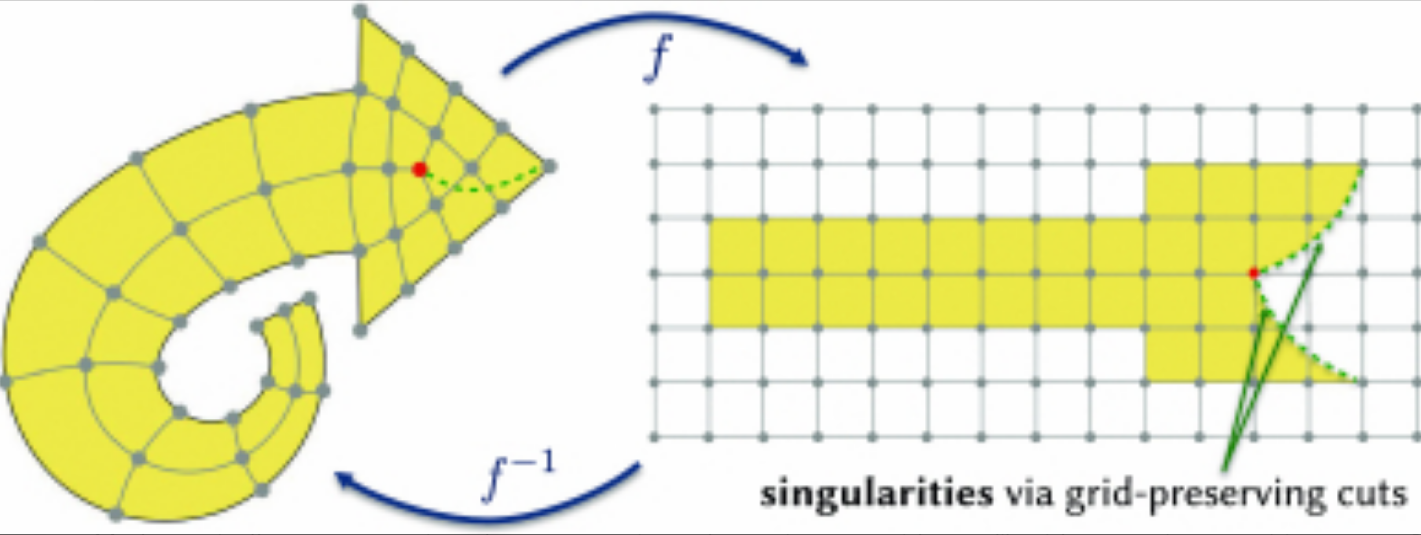
\includegraphics[width=20em]{figures/integer-grid-rough}
  \caption{Idea of quadrangulation with integer-grid maps in 2D (Figure from \cite{Hex22})}
  \label{fig:integer-grid}
\end{figure}
This is called an integer-grid map and by minimizing distortion and satisfying boundary alignment,
a hexahedral mesh could be extracted.
However, this is a hard mixed-integer and non-convex optimization problem for which no current
optimization technique is available that would result in an acceptable solution.

\subsection{Frame fields as a relaxation}
By taking the Jacobian of the parametrization, $\nabla \phi$, we get a mapping
$\nabla \phi : \mathcal{M} \to \mathbb{R}^{3\times3}$ of \emph{frames}, a \emph{frame field}.
The idea of frame fields is then to search for an approximation of $\nabla \phi$.
If $F: \mathcal{M} \to \mathbb{R}^{3\times3}$ is the approximation of $\nabla \phi$, we can
solve for $\phi : \mathcal{M} \to \mathbb{R}^3$ with
$$\min \limits_{\phi} \int \limits_{\mathcal{M}} ||\nabla \phi F - \Id||^2$$
where $||\cdot||$ is the Frobenius norm. If this is sufficiently small, then $F^{-1} \approx \nabla \phi$ and 
the extracted hexahedral mesh closely follow the integer-grid isolines.
A frame locally represents the edges of a deformed cube.
We can think of a frame field as the composition of three vector fields
and as a relaxation of the original problem. However, frame fields
can contain singularities that the underlying vector fields do not contain \cite{Nieser}
and contain types of singularities that cannot appear in hex meshes \cite{Liu}.
These singularities are said to be non-meshable.
The problem of non-meshability is not discussed further here, but it
is something to be aware of.

We treat a frame $F$ as a set of 3 linearly independent vectors $\{F_1,F_2,F_3 \}$ which we can
collect into a matrix $F=(F_1,F_2,F_3) \in \mathbb{R}^{3\times 3}$.
Notice that many of these frames are equivalent.
There are $2^3$ choices of the sign, and $3!$ possible permutations, which
gives $2^3\cdot 3! = 48$ equivalent frames.
Since we want non-degenerate frames and the same orientation through the grid, the constraint $\det(F)>0$ is imposed,
which leaves $24$ equivalent frames.
Equivalence of frames is then defined as
$$F_u \sim F_v \iff \exists R \in \mathcal{O} : F_u=RF_v$$
where $\mathcal{O}$ is the \emph{chiral cubical symmetry group}\cite{Nieser}.
These symmetries make the optimization for frame fields more complicated.
To handle these symmetries, we use the spherical harmonics based representation \cite{Huang}.
The idea is to use the polynomial $x^4+y^4+z^4$ to express the frames as rotations.
Under the restriction of the polynomial to the sphere, that is $\mathbb{S}^2\to \mathbb{R}$, the octahedral frames
are invariant under the chiral cubical symmetry group. However, the spherical harmonics
manifold is 9-dimensional, so not all vectors in the spherical harmonics represent valid frames,
since rotations only exhibit 3 degrees of freedom.
While optimizing the frame field, some kind of ``average'' of two frames will be done.
This averaging makes sense in the spherical harmonics space, but the result may be outside the valid
space of frames. A projection from the spherical
harmonics space back to the valid space of frames will be needed, see fig. \ref{fig:projection} \cite{Ray}.
\begin{figure}[htb]
  \centering
  \def\svgwidth{20em}
  \input{figures/projection.pdf_tex}
  \caption{Combination of two valid frames leads to a resulting frame outside the valid frames. A projection to the nearest valid frame is done.}
  \label{fig:projection}
\end{figure}


When a frame $F$ has orthonormal columns, the resulting hex elements look like unit cubes.
By introducing a metric $g$, we can control the size and shear of the cubes by
relaxing the orthonormality constraint to $g$-orthonormality when
$$F^{-1}gF = \Id$$
holds. We can decompose the frame field $F$ into a rotational part $R : \mathcal{M} \to \text{SO}(3)$ and a symmetric metric part $g^{-1/2}$
(akin to the polar decomposition of linear transformations)\cite{Panozzo}, that is $F = g^{-1/2}R$,
see figure \ref{fig:factorization}.

\begin{figure}[htb]
  \centering
  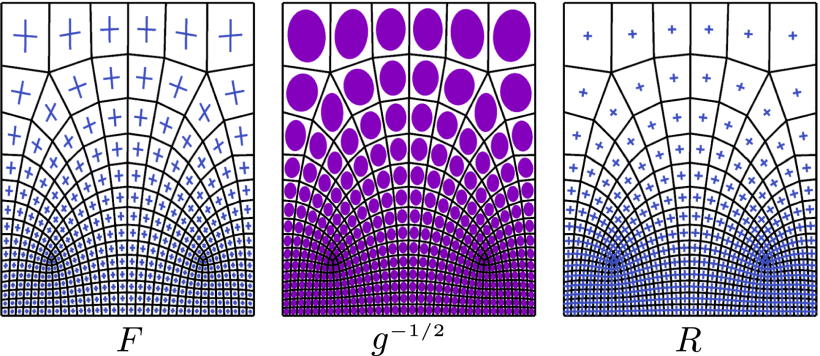
\includegraphics[width=25em]{figures/factorization}
  \caption{Factorization of a $g$-orthogonal frame field into a symmetric metric part $g^{-1/2}$ and a rotational part $R$
  (Figure from \cite{Fang23}).}
  \label{fig:factorization}
\end{figure}

TODO:
Frame field goals

\begin{itemize}
  \item Dirichlet energy, what are we optimizing
  \item Requirements for the frame field -> integrability + boundary alignment
\end{itemize}




\end{document}